In this section we investigate LFA of two preconditioners often used as smoothers for multigrid methods.
These smoothers can also be used as preconditioners for iterative solvers independently from multigrid methods.

The error propagation operator for a preconditioner is given by $\mathbf{S} = I - \mathbf{M}^{-1} {\color{burgundy}\mathbf{A}}$, where $\mathbf{M}^{-1}$ is determined by the particular preconditioner under investigation.
We will define the symbol of the error propagation operator for weighted Jacobi preconditioner and the Jacobi preconditioned Chebyshev semi-iterative method.

The LFA-predicted convergence factor is given by the maximum spectral radius of the symbol of the error propagation operator across all frequencies
\begin{equation}
\mu = \max_{\boldsymbol{\theta} \in T^{\text{low}}, T^{\text{high}}} \rho \left( \tilde{\mathbf{S}} \left( \nu, \omega, \boldsymbol{\theta} \right) \right),
\end{equation}
where $ \rho \left( \tilde{\mathbf{S}} \left( \nu, \omega, \boldsymbol{\theta} \right)\right)$ denotes the spectral radius of the matrix symbol $\tilde{\mathbf{S}}$.

\begin{figure}[!ht]
  \centering
  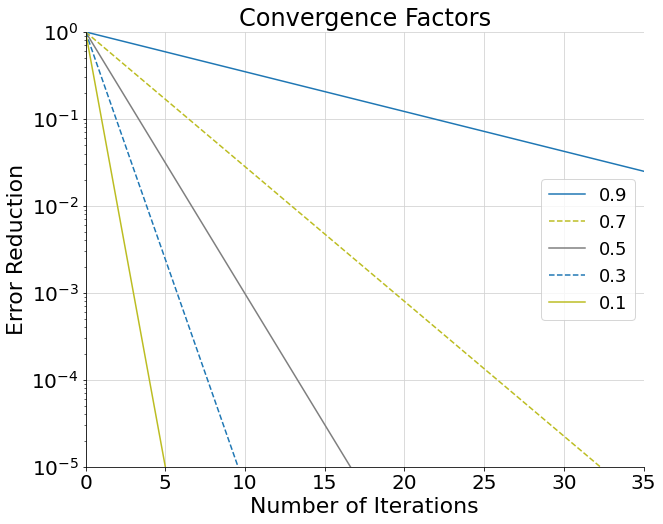
\includegraphics[width=0.55\textwidth]{../img/convergenceFactors}
  \caption{Iterations Required to Target Error Tolerances}
  \label{fig:error_tolerance}
\end{figure}

\begin{table}[ht!]
\begin{center}
\begin{tabular}{l c c c c c}
  \toprule
  Tolerance   &  $\rho = 0.9$  &  $\rho = 0.7$  &  $\rho = 0.5$  &  $\rho = 0.3$  &  $\rho = 0.1$  \\
  \toprule
  $10^{-1}$   &  $22$          &  $7$           &  $4$           & $2$            &  $1$           \\
  $10^{-5}$   &  $110$         &  $33$          &  $17$          & $10$           &  $5$           \\
  $10^{-10}$  &  $219$         &  $65$          &  $34$          & $20$           &  $10$          \\
  $10^{-15}$  &  $328$         &  $97$          &  $50$          & $29$           &  $15$          \\
  \bottomrule
\end{tabular}
\end{center}
\caption{Iterations Required to Target Error Tolerances}
\label{table:error_tolerance}
\end{table}

If we consider a Richardson iteration as an iterative solver for a system of equations, then the convergence factor for a preconditioner or smoother determines how many iterations would be required for the Richardson iteration to reach a target reduction in error.
Table \ref{table:error_tolerance} shows the number of iterations required to achieve a range of target error tolerances for different convergence factors.
Figure \ref{fig:error_tolerance} shows this same information in a visual format to emphasize the importance of reducing the convergence factor for these methods.

Note that Krylov subspace methods, such as the Conjugate Gradient (CG) method, converge faster than Richardson iterations; however, this convergence factor still provides valuable information about the effectiveness of these preconditioners.
A smaller convergence factor indicates that the preconditioned operator is closer to the identity operator, which indicates that CG iterations will converge much faster.

% -- Jacobi -------------------------------------------------------------------
\subsection{Jacobi}
\input 03-LocalFourierAnalysis/02-01-jacobi

% -- Chebyshev ----------------------------------------------------------------
\subsection{Chebyshev}
\input 03-LocalFourierAnalysis/02-02-chebyshev